\subsection{RQ3: Revision in test and production methods}
Prior studies have shown that test code does not evolve as consistently as production code~\cite{zaidman2011studying,levin2017co}. Test maintenance often lags behind production changes, and many production-code modifications are performed without corresponding updates to the test suite. For many projects, fewer than 15\% of commits involve test maintenance~\cite{levin2017co}, and even popular open-source projects may experience limited testing activity~\cite{marsavina2014studying}. Furthermore, when test methods are modified, such changes are often assumed to be triggered by changes in the corresponding production methods~\cite{sun_revisiting_2023,hu2023identify}. While test code can evolve alone due to its own internal problems, such as smells, that is also true for production code. Collectively, these observations suggest that test code should evolve less frequently than production code. In this section, leveraging accurate method-level history tracking (RQ1) and mapping (RQ2), we empirically evaluate this assumption by comparing the revision characteristics of test and production methods. 

\subsubsection{Approach}
As \emph{HistoryFinder} achieved the best performance for tracking both production code~\cite{islam_historyfinder_2025} and test code (RQ1), we used it to collect revision histories for all methods in the 110 projects described in Section~\ref{setup}. After filtering helper test methods as well as getter and setter methods from the production code (Section~\ref{setup}), we collected the revision histories of 1,760,423 production methods and 567,904 test methods. Although \emph{HistoryFinder} reports a revision when the containing file of a method is renamed, even if the method itself remains unchanged, we excluded such revisions from our dataset. The complete project-level statistics are available in the replication repository (\texttt{data/rqs/rq3/method-count.csv}).
% \footnote{\href{https://github.com/SQMLab/method-co-evolution/blob/main/data/rqs/rq3/method-count.csv}{/data/rqs/rq3/method-count.csv}}


% \begin{figure*}[htbp]
% \setlength{\belowcaptionskip}{-10pt}

% \centering
% \mbox{
% \subfigure[]{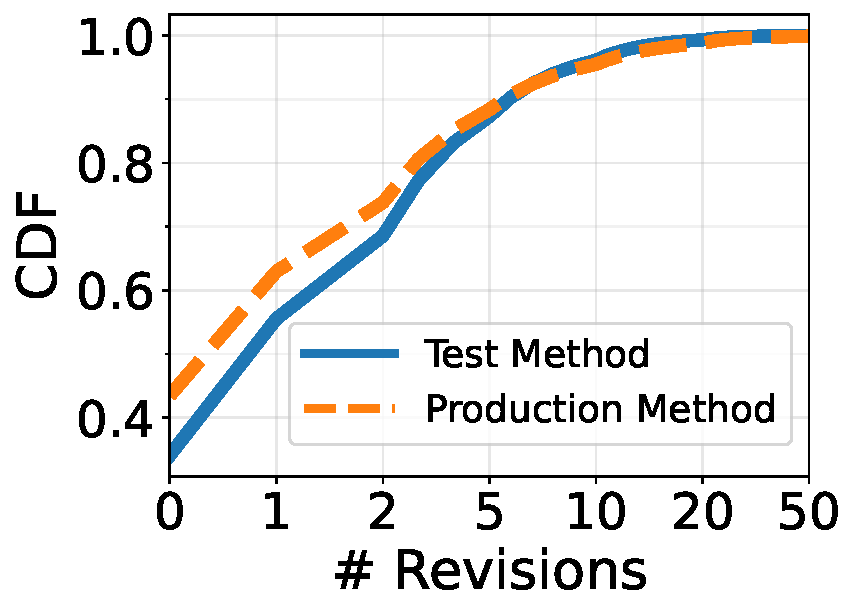
\includegraphics[width=0.28\textwidth,keepaspectratio]{figure/artifact-revision-cdf--historyFinder.pdf}}
% \subfigure[]{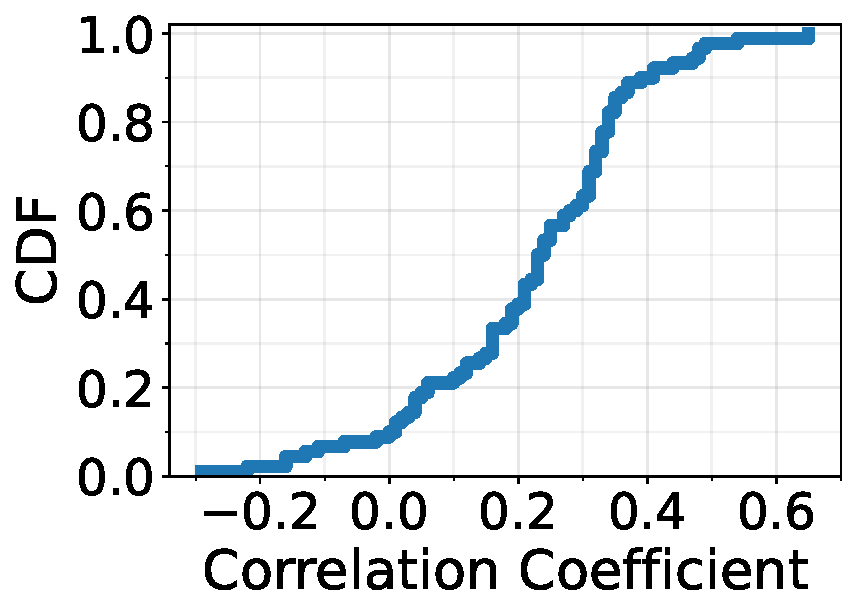
\includegraphics[width=0.28\textwidth,keepaspectratio]{figure/t2p-correlation-cdf--historyFinder--omc--nc.pdf}}
% \subfigure[]{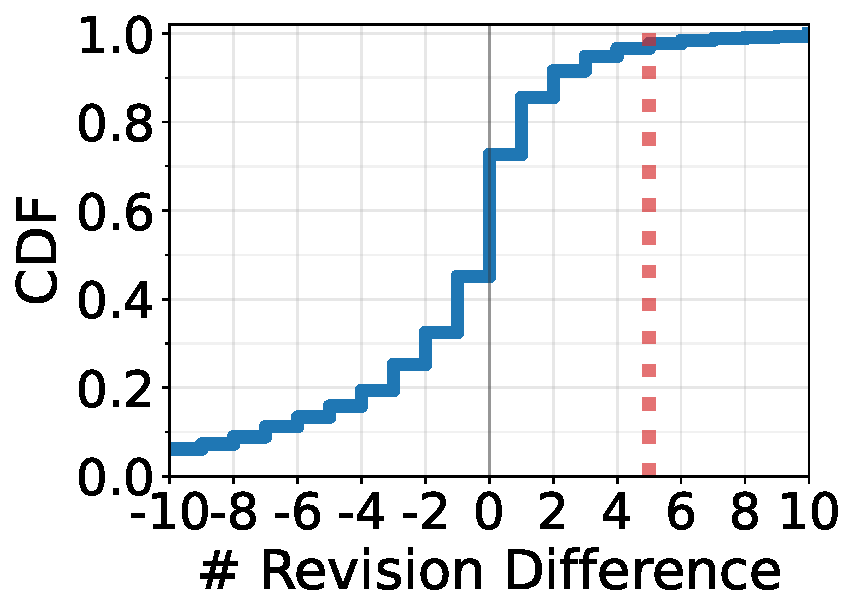
\includegraphics[width=0.28\textwidth,keepaspectratio]{figure/t2p-revision-delta-cdf--historyFinder--omc--nc.pdf}}
% }

% \caption{Figure (a) shows the CDF of the number of revisions for both production and test methods. To enhance readability, we restricted the x-axis to 50. Figure (b) shows the CDF of correlation coefficients between the number of revisions in test methods and their corresponding production methods. Figure (c) shows the CDF of differences in revisions between test methods and their corresponding production methods. It is important to note that all test and production methods were used for Figure (a), while only mapped examples were used for (b) and (c).}
% % \textcolor{red}{the label of a and c is problematic.. For a, the x-label should be \# Revisions, for c, the level should be Revision difference. Also, the figures don't match in shape.. Remove the legend from figure c}
% \label{fig:revisions}
% \end{figure*}

\begin{figure*}[htbp]
\centering
\setlength{\belowcaptionskip}{-10pt}

\begin{subfigure}[t]{0.31\textwidth}
    \centering
    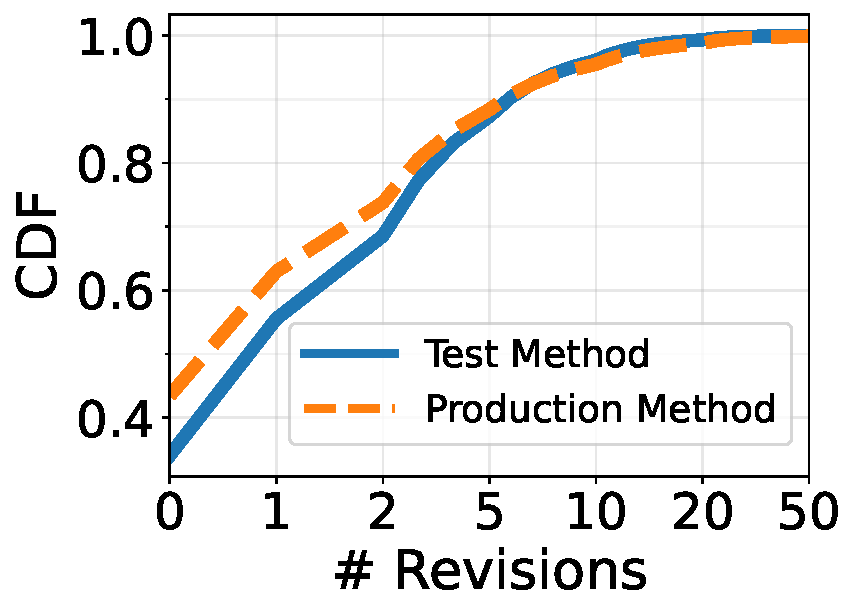
\includegraphics[width=\linewidth,keepaspectratio]{figure/artifact-revision-cdf--historyFinder.pdf}
    \caption{}
    \label{fig:revisions-a}
\end{subfigure}
\hfill
\begin{subfigure}[t]{0.31\textwidth}
    \centering
    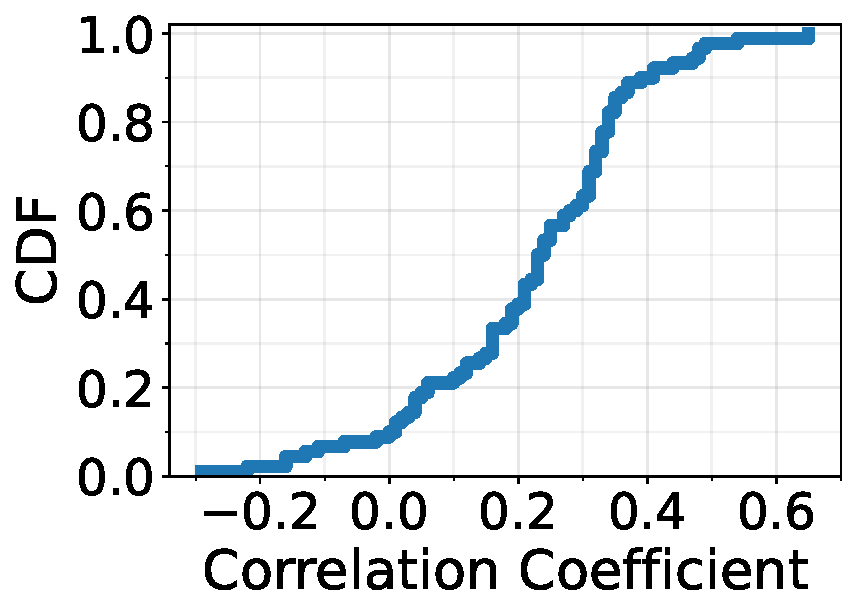
\includegraphics[width=\linewidth,keepaspectratio]{figure/t2p-correlation-cdf--historyFinder--omc--nc.pdf}
    \caption{}
    \label{fig:revisions-b}
\end{subfigure}
\hfill
\begin{subfigure}[t]{0.31\textwidth}
    \centering
    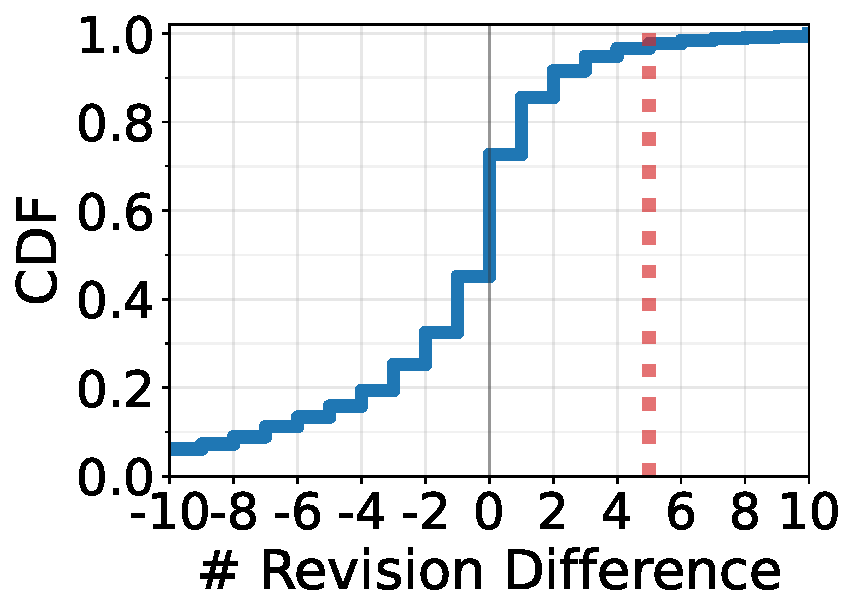
\includegraphics[width=\linewidth,keepaspectratio]{figure/t2p-revision-delta-cdf--historyFinder--omc--nc.pdf}
    \caption{}
    \label{fig:revisions-c}
\end{subfigure}

\caption{Figure (a) shows the CDF of the number of revisions for both production and test methods. To enhance readability, we restricted the x-axis to 50. Figure (b) shows the CDF of correlation coefficients between the number of revisions in test methods and their corresponding production methods. Figure (c) shows the CDF of differences in revisions between test methods and their corresponding production methods. It is important to note that all test and production methods were used for Figure (a), while only mapped examples were used for (b) and (c).}
\label{fig:revisions}
\end{figure*}

When production-to-test mappings were required, we prioritized precision over recall because we need reliable links for reliable analysis. Also, given our large number of projects and methods, even a lower-recall approach can produce a sufficiently large sample for reliable statistical analysis, provided that the mappings are accurate. Therefore, based on the findings of RQ2, we adopted the \emph{OMC+NC} approach, which provides substantially higher recall than \emph{NC} while incurring a small reduction in precision. For example, for the \emph{all} dataset, the precisions of \emph{NC} and \emph{OMC+NC} are 0.95 and 0.89, respectively. However, the recall of \emph{NC} is only 0.09 in contrast to 0.22 of \emph{OMC+NC}.

% \footnote{\url{https://github.com/shahidul2k9/method-co-evolution/blob/main/data/research-question/rq3/artifact-revision-mww--historyFinder.pdf}}

% The baseline method-level comparison includes 1,182,344 test methods. It also
% includes 2,152,609 production methods.

% by utilizing the HistoryFinder tool~\cite{}.  because RQ1
% shows that it provides the strongest overall accuracy for test-method history
% reconstruction.  The analysis includes concrete methods only.  As a baseline
% method-level comparison, we compare test methods with production methods.  We
% visualize their revision distributions with CDFs and, for each project,
% compare the distributions using a two-sided
% Mann--Whitney U test and Cliff's~$\delta$. 

% We count a revision only when the corresponding commit contains an actual
% source-code difference within the method.  We exclude the method-introduction
% commit, so a value of zero means that the method was introduced but not later
% changed in a source-modifying commit.  File moves, file renames, and method
% moves without implementation changes are therefore not counted as revisions.

% Using the \textit{omc--nc} strategy from RQ2, we link test methods to the
% production methods they exercise. We then compare the number of revisions made
% to each linked test method with the number of revisions made to its production
% method. Based on the difference between test method revisions and production
% method revisions, we define three revision-difference groups:
% \textbf{Normal Test Revision (NTR)} when test method revisions are less than or
% equal to production method revisions, \textbf{Moderate Test Revision (MTR)}
% when test method revisions exceed production method revisions by one to four,
% and \textbf{High Test Revision (HTR)} when test method revisions exceed
% production method revisions by five or more.

% \begin{table*}[htbp]
% \centering
% \caption{ We report the $p-value$ from the Wilcoxon rank sum test, as well as Cliff's delta effect size with sign. To save space,
% we only show results for a few projects. The complete list of project-level comparisons is available in the replication repository.\protect\footnotemark}

% Two-sided Mann--Whitney U test comparing the number of revisions of \textbf{production} methods versus \textbf{test} methods
% per project.
% Each row reports the two-sided $p$-value, Cliff's~$\delta$ effect size ($d$), and its
% direction sign: \textbf{$+$}~(43~project(s)) indicates that production methods
% have a higher revision count than test methods ($\delta > 0$);
% \textbf{$-$}~(66~project(s)) indicates the opposite,
% i.e.\ test methods are revised more frequently ($\delta < 0$).
% Effect size bands follow Romano et al.\ thresholds for Cliff's~$\delta$: \textbf{N}~negligible ($|\delta| < 0.147$), \textbf{S}~small ($0.147 \le |\delta| < 0.33$), \textbf{M}~medium ($0.33 \le |\delta| < 0.474$), \textbf{L}~large ($|\delta| \ge 0.474$). 


% \label{tab:artifact-revision-mww}
% \begin{tabular}{l r r c c c c c}
\toprule
\textbf{Project} & \textbf{P-value} & \textbf{Sign} &  & \multicolumn{4}{c}{\textit{\textbf{Effect size}}} \\
\cmidrule(l){5-8}
 & & & +/- & N & S & M & L \\
\midrule
Activiti & 0.00 & -0.13 & - & x &  &  &  \\
ant & 0.00 & 0.38 & + &  &  & x &  \\
AntennaPod & 0.34 & 0.03 & + & x &  &  &  \\
.................\\
Apktool & 0.00 & -0.21 & - &  & x &  &  \\
argouml & 0.01 & 0.06 & + & x &  &  &  \\
\bottomrule
\end{tabular}

% \end{table*}
% \footnotetext{\url{https://github.com/shahidul2k9/method-co-evolution/blob/main/data/research-question/rq3/artifact-revision-mww--historyFinder.pdf}}



\subsubsection{Result}
Figure~\ref{fig:revisions} (a) shows the cumulative distribution function (CDF) of revisions for production and test methods after aggregating data across all projects. Surprisingly, test methods underwent more revisions than production methods when comparing low change-prone methods (0 to 2 revisions). For example, more than 62\% of test methods were revised at least once, compared with approximately 56\% of production methods. The non-parametric Wilcoxon rank-sum test~\cite{dzidek2008realistic,chowdhury_evidence_2025} shows this difference to be significant ($p$-value $\leq 0.05$). 
We also performed the analysis at the project level and found that test methods were revised more frequently than production methods in 65 projects, with statistically significant differences in 55 projects. The corresponding Cliff's delta effect sizes~\cite{Zhang:2013} were negligible, small, medium, and large in 41.8\%, 40\%, 12.7\%, and 5.5\% of the projects, respectively. In contrast, production methods were revised more frequently in 43 projects, with statistically significant differences in 36 projects. The full table is available with our replication package (\texttt{/data/rqs/rq3/revision-statistics.pdf}).
% \footnote{\href{https://github.com/SQMLab/method-co-evolution/blob/main/data/rqs/rq3/revision-statistics.pdf}{/data/rqs/rq3/revision-statistics.pdf}}

For each project separately, using the mapped production-to-test examples, we calculated Kendall's $\tau$ correlation coefficient~\cite{Inozemtseva:2014} between the number of revisions of test methods and the number of revisions of their corresponding production methods. Figure~\ref{fig:revisions} (b) shows that, for 60\% of the projects, the coefficients are below 0.3. This finding contrasts with the common assumption that test methods are revised primarily in response to changes in their corresponding production methods. Under this assumption, one would expect co-evolution between production and test methods and, consequently, a strong correlation in their revision frequencies.

To investigate more, we used the mapped test and production samples again to calculate the revision difference between test methods and their corresponding production methods. Figure~\ref{fig:revisions} (c) shows that, in only 45\% of the cases, production methods were revised more frequently than their test methods. In 26\% of the cases, the number of revisions was identical. For the remaining 29\% cases, test methods were revised more than their corresponding production methods. Notably, more than 3\% of test methods were revised at least five more times than their corresponding production methods.
% \begin{figure}[htbp]
%     \centering
%     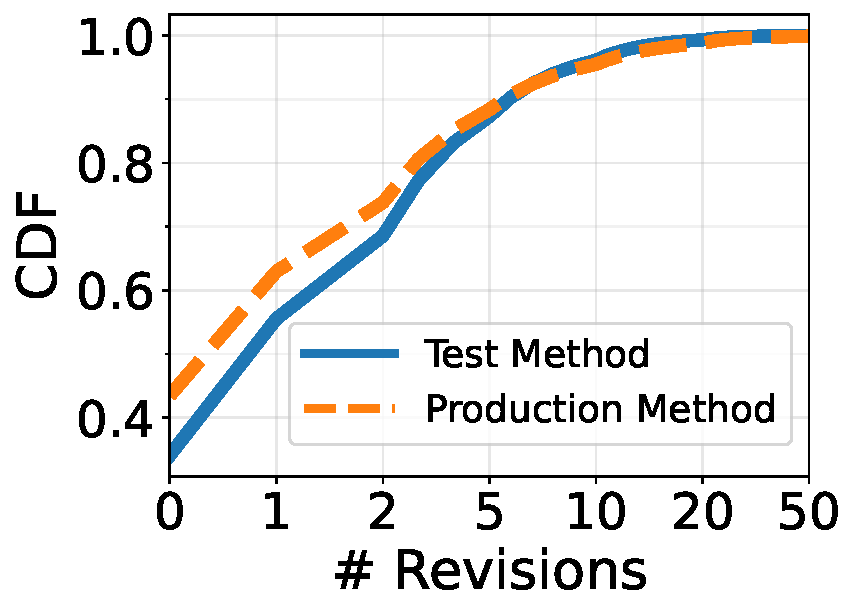
\includegraphics[width=0.7\linewidth]{figure/artifact-revision-cdf--historyFinder.pdf}
%     \caption{ \textcolor{red}{the x-axis label should be \# Revisions.. }}
%     \label{fig:rq3-artifact-revision-cdf}
% \end{figure}



% \begin{figure*}[htbp]
%     \centering
%     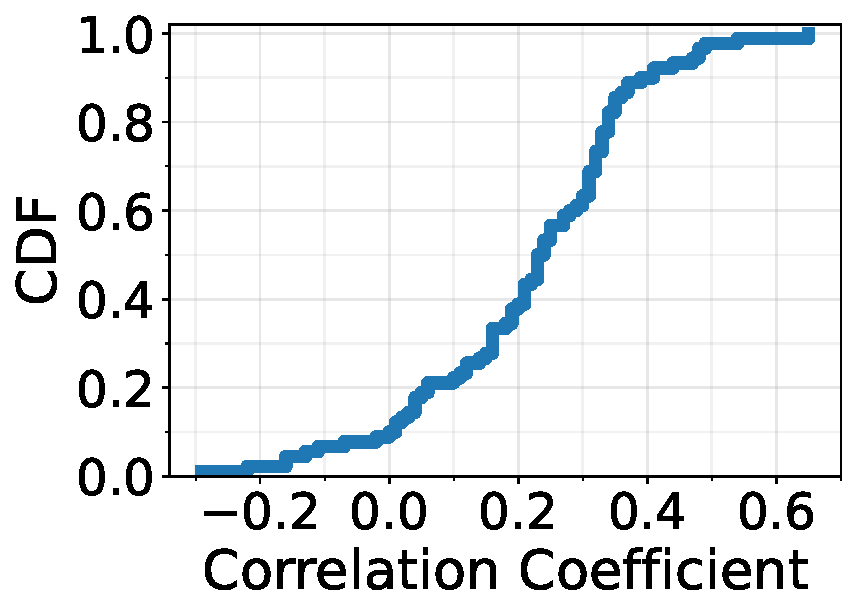
\includegraphics[width=.4\textwidth]{figure/t2p-correlation-cdf--historyFinder--omc--nc.pdf}
%     \hfill
%     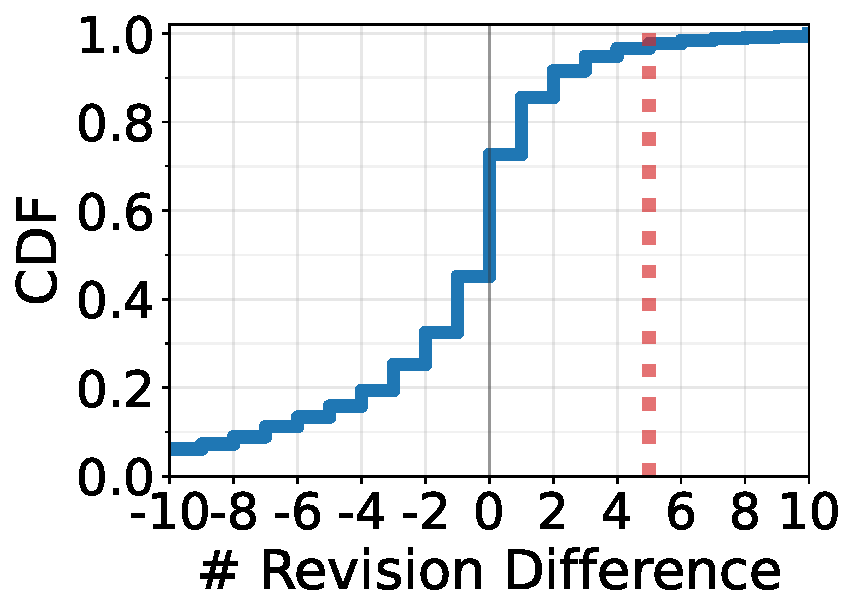
\includegraphics[width=.4\textwidth]{figure/t2p-revision-delta-cdf--historyFinder--omc--nc.pdf}
%     \caption{Linked test--production method revision relationship for the
%     \textit{omc--nc} strategy. Left: CDF of project-level revision correlation
%     coefficients. Right: CDF of test-minus-production revision differences,
%     with NTR, MTR, and HTR summarizing the revision-difference groups.}
%     \label{fig:rq3-t2p-revision-relation}
% \end{figure*}

% Figure~\ref{fig:revisions} (a) shows the cumulative distribution function (CDF) of the number of revisions for both production and test methods, after aggregating data from all projects. To our surprise, with the aggregated data, we see that test methods observe more revisions than source methods. For example, more than 65\% of the test methods were revised at least once, which is true for approximately 56\% of the production methods. \textcolor{red}{We used the non-parametric Wilcoxon rank sum test and found that this difference is statistically significant ($p-value \le 0.05$). Also, the non-parametric Cliff's delta shows X effect size. We evaluated this at the project level as well, presented in Table~\ref{tab:artifact-revision-mww}, and found that in 66 projects, test methods were revised more than source methods with statistical significance in X projects, and with effect sizes negligible, small, and medium in X\%, y\%, and z\% of the projects, respectively.  In contrast, production methods were revised more in 43 projects with statistical significance in Y projects.} 

% After mapping between the test and production methods, we lost many samples due to the low recall of the \emph{NC+OMC} approach. \textcolor{red}{With the X number of production-to-test mapped examples}, we calculated the Kendall's $\tau$ correlation coefficient between the number of revisions of test methods and the number of revisions for their corresponding production methods. We calculated this for each project separately, producing 109 correlation coefficient values. Figure~\ref{fig:revisions} (b) shows that for 60\% of projects, the coefficients are below 0.3. This indicates a potential contrast to the common assumption that test methods are revised mainly in response to changes in their production methods. 

% To verify even further, we calculated the revision difference between the test and their production methods. Figure~\ref{fig:revisions} (c) shows that for 45\% of the cases, production methods were revised more than their test methods. For 26\% cases, the number of revisions was equal. The remaining 29\% test methods were revised more than their production methods. More than 3\% test methods were revised at least five times more than their production methods. 

% For easy reference, we call these test methods NTR (normal test revision).   

% that their post-introduction
% revision distributions are closely aligned.  Thus, test methods are not merely
% static validation material; they are revised at a scale comparable to
% production methods.

% The project-level Mann--Whitney U results reinforce that the practical
% separation is usually limited. Across 109 project-level comparisons, production
% methods have higher revision counts in 58 projects, test methods have higher
% counts in 50 projects, and one project is tied. Although 91 comparisons are
% statistically significant, the effect sizes are mostly small in practice: 62
% comparisons are negligible, 35 are small, 11 are medium, and one is large. Even
% among the statistically significant comparisons, 46 are negligible and 33 are
% small. Thus, project-level differences are common, but large practical
% differences are uncommon.


% The direct test--production comparison gives a more specific answer.
% The baseline method-level comparison does not show whether test revisions are
% explained by the production methods under test, so
% Figure~\ref{fig:rq3-t2p-revision-relation} examines linked pairs.  The
% correlation CDF shows that linked test and production revisions are usually
% positively related, but not perfectly synchronized.  The revision-difference
% CDF shows that most linked test methods are revised no more frequently than the
% production methods they exercise: $71{,}368$ pairs (72.7\%) fall into NTR.  The
% exceptions are also important: $23{,}517$ pairs (24.0\%) fall into MTR, and
% $3{,}275$ pairs (3.3\%) fall into HTR.

% Thus, test methods are generally not revised more frequently than their linked
% production methods, but a non-trivial minority does outpace production
% revisions.  HTR is rare but important because it captures excess test
% maintenance that cannot be explained solely by revisions to the production
% method under test.  This subset provides the target population for RQ4, where
% we examine whether initial test smells are associated with such excess test
% maintenance.

\begin{framed}
\noindent\textbf{\underline{RQ3 summary}:}
Leveraging accurate test method history tracking and production-to-test mappings, we find that in many projects, test methods undergo more revisions than their corresponding production methods. 
\end{framed}
